%From https://egu2018.eu/PICO_how-to_guide_to_PICO.pdf
%Abstracted and templated by Brian Ballsun-Stanton, Macquarie University.
%original template by https://github.com/snowtechblog/pico-latex-presentation by Anselm Köhler

\documentclass[unknownkeysallowed,usepdftitle=false, parskip=full, aspectratio=169]{beamer}
% unknownkeysallowed is needed for mac and the newer latex version -> is more picky than before...
\usetheme[headheight=1cm,footheight=2cm]{boxes}
%\usetheme{default}


\usepackage{default}
\usepackage{graphicx}
%example pictures created via: http://lorempixel.com/1200/800/cats/Figure2/. Credit to http://lorempixel.com/images.php

\usepackage{epsfig}
\usepackage{siunitx}
\usepackage{color}
\usepackage{ifthen}
%usepackage{ragged2e}

\usepackage[T1]{fontenc}
\usepackage[utf8]{inputenc}
%https://tex.stackexchange.com/a/203804/5483

\usepackage[activate={true,nocompatibility},final,tracking=true,kerning=true,spacing=true,factor=1100,stretch=10,shrink=10]{microtype} % http://www.khirevich.com/latex/microtype/
\microtypecontext{spacing=nonfrench}

\usepackage{lipsum} % for dummy text only
\usepackage[UKenglish]{babel} %https://tex.stackexchange.com/a/27743 
\usepackage[pangram]{blindtext} % https://tex.stackexchange.com/a/48411

%\usepackage{parskip} % from https://tex.stackexchange.com/q/11622
%\setlength{\parskip}{12pt} 

%\setparsizes{\parindent}{12pt}{\parfillskip}

%\usepackage{etoolbox} % as per https://tex.stackexchange.com/a/24331
%\appto\chapterheadendvskip{\vspace{-1\parskip}}
%\setparsizes{\parindent}{50pt plus 20pt minus 30pt}{\parfillskip}

\setbeamertemplate{navigation symbols}{}%remove navigation symbols
\setbeamersize{text margin left=1cm,text margin right=1cm}

% some colors
\definecolor{grau}{gray}{.5}
\definecolor{slfcolor}{rgb}{0,0.6274,0.8353}
\definecolor{wslcolor}{rgb}{0,0.4,0.4}

% setup links
\hypersetup{%
	%linkbordercolor=green,%
	colorlinks=false,%
	pdfborderstyle={/S/U/W 0},%
	%pdfpagemode=FullScreen,%
	pdfstartpage=4%
	}

% setup some fonts
\setbeamerfont{title}{series=\bfseries, size=\small}
\setbeamerfont{author}{size*={5pt}{0pt}}
\setbeamerfont{institute}{size*={3pt}{0pt}}
\setbeamerfont{bodytext}{size=\scriptsize}
\setbeamerfont{caption}{size*={0.1pt}{0.0pt}}
	
% Title setup	
\title{Improving Your Research Process Through Tools}
\author{Osmond Chiu\inst (\texttt{osmond.chiu@student.mq.edu.au})}
\institute{Macquarie University}
% add title in headbox
\setbeamertemplate{headline}
{\leavevmode
\begin{beamercolorbox}[width=1\paperwidth]{head title}
  % LOGO
  \vspace{0.1cm}
  \begin{columns}[t, totalwidth=\textwidth]
  \begin{column}[c]{1.05cm}
  \end{column}
  % TITLE
   \begin{column}[c]{10.6cm}
   \centering \usebeamerfont{title} \textcolor{red}{\inserttitle} \\
   \centering \usebeamerfont{author} \color[rgb]{0,0,0} \insertauthor \\
   \vspace{-0.05cm}
   \centering \usebeamerfont{institute} \insertinstitute
  \end{column}
  % PICTURE
  \begin{column}[c]{1.15cm}
    \hspace{0.005cm}
  \end{column}
  \end{columns}
  {\color{red}\hrule height 1pt\vspace{0.1cm}}
\end{beamercolorbox}%
}

% setup the navigation in footbox
% first set some button colors
\newcommand{\buttonactive}{\setbeamercolor{button}{bg=red,fg=white}}
\newcommand{\buttonpassive}{\setbeamercolor{button}{bg=red,fg=black}}
% now set up that the one active one gets the new color.
\newcommand{\secvariable}{nothing}
% therefore we write before each section (well, everything which should be part of the navi bar)
% the variable \secvariable to any name which is in the next function ...
\newcommand{\mysection}[1]{\renewcommand{\secvariable}{#1}
}
% ... compaired to strings in the following navibar definition ...
\newcommand{\tocbuttoncolor}[1]{%
 \ifthenelse{\equal{\secvariable}{#1}}{%
    \buttonactive}{%
    \buttonpassive}
 }
% ... here we start to set up the navibar. each entry is calling first the function \tocbuttoncolor with the argument which should be tested for beeing active. if active, then change color. afterwards the button is draw. so to change that, you need to change the argument in \toc..color, the first in \hyperlink and before each frames definition... A bit messed up, but works...
\newlength{\buttonspacingfootline}
\setlength{\buttonspacingfootline}{-0.2cm}
\setbeamertemplate{footline}
{\leavevmode
\begin{beamercolorbox}[width=1\paperwidth]{head title}
  {\color{red}\hrule height 1pt}
  \vspace{0.05cm}
  % set up the buttons in an mbox
  \centering \mbox{
    \tocbuttoncolor{abstract}
    \hyperlink{abstract}{\beamerbutton{2 Min Madness}}
    \tocbuttoncolor{radar}
    \hspace{\buttonspacingfootline}
      \hyperlink{radar}{\beamerbutton{Functions}}

    \tocbuttoncolor{line}
    \hspace{\buttonspacingfootline}
      \hyperlink{line}{\beamerbutton{VirtualBox}}
    \tocbuttoncolor{major}
    \hspace{\buttonspacingfootline}
      \hyperlink{major}{\beamerbutton{Open Semantic}}
    \tocbuttoncolor{slab}
    \hspace{\buttonspacingfootline}
      \hyperlink{slab}{\beamerbutton{Zotero}}
    \tocbuttoncolor{minor}
    \hspace{\buttonspacingfootline}
      \hyperlink{minor}{\beamerbutton{Hypothes.is}}
    \tocbuttoncolor{conclusion}
    \hspace{\buttonspacingfootline}
      \hyperlink{conclusion}{\beamerbutton{Conclusion}}
    % this last one should normaly not be used... it will open the preferences to change the 
    % behaviour of the acrobat reader in fullscreen -> usefull in pico...
    \setbeamercolor{button}{bg=white,fg=black}
    % for presentation
    %\hspace{-0.1cm}\Acrobatmenu{FullScreenPrefs}{\beamerbutton{\#}}
    % for upload
    
     
\Acrobatmenu{FullScreenPrefs}{\vspace{0.3cm}\hspace{0.24cm}\mbox{%
      
\includegraphics[height=0.04\textheight,keepaspectratio]{%
	  figure/CreativeCommons_Attribution_License.eps}%
	  }}
   }
    \vspace{0.05cm}
\end{beamercolorbox}%
}


\begin{document}


%%%%%%%%%%%%%%%%%%%%%%%%%%%%%%%%%%%%%%%%%%%%%%%%%%%%%%%%%%%%%%%%%%%%%%%%%%
\mysection{abstract}
%%%%%%%%%%%%%%%%%%%%%%%%%%%%%%%%%%%%%%%%%%%%%%%%%%%%%%%%%%%%%%%%%%%%%%%%%%
\begin{frame}\label{\secvariable}

\usebeamerfont{bodytext}


\parbox{\linewidth}{

\begin{columns}[t]
    \begin{column}[c]{0.5\textwidth}

Organising sources and managing references are two common and time consuming tasks when doing research

 \vspace{12pt}

Common problems with these tasks:
\begin{itemize}
\item Can't remember relevant source
\item Can't remember key line in source
\item Can't recall the topics covered in a source
\item Need to double check citations
\item Need to keep track of references for a bibliography
\end{itemize}

 \end{column}
    \begin{column}[c]{0.5\textwidth}
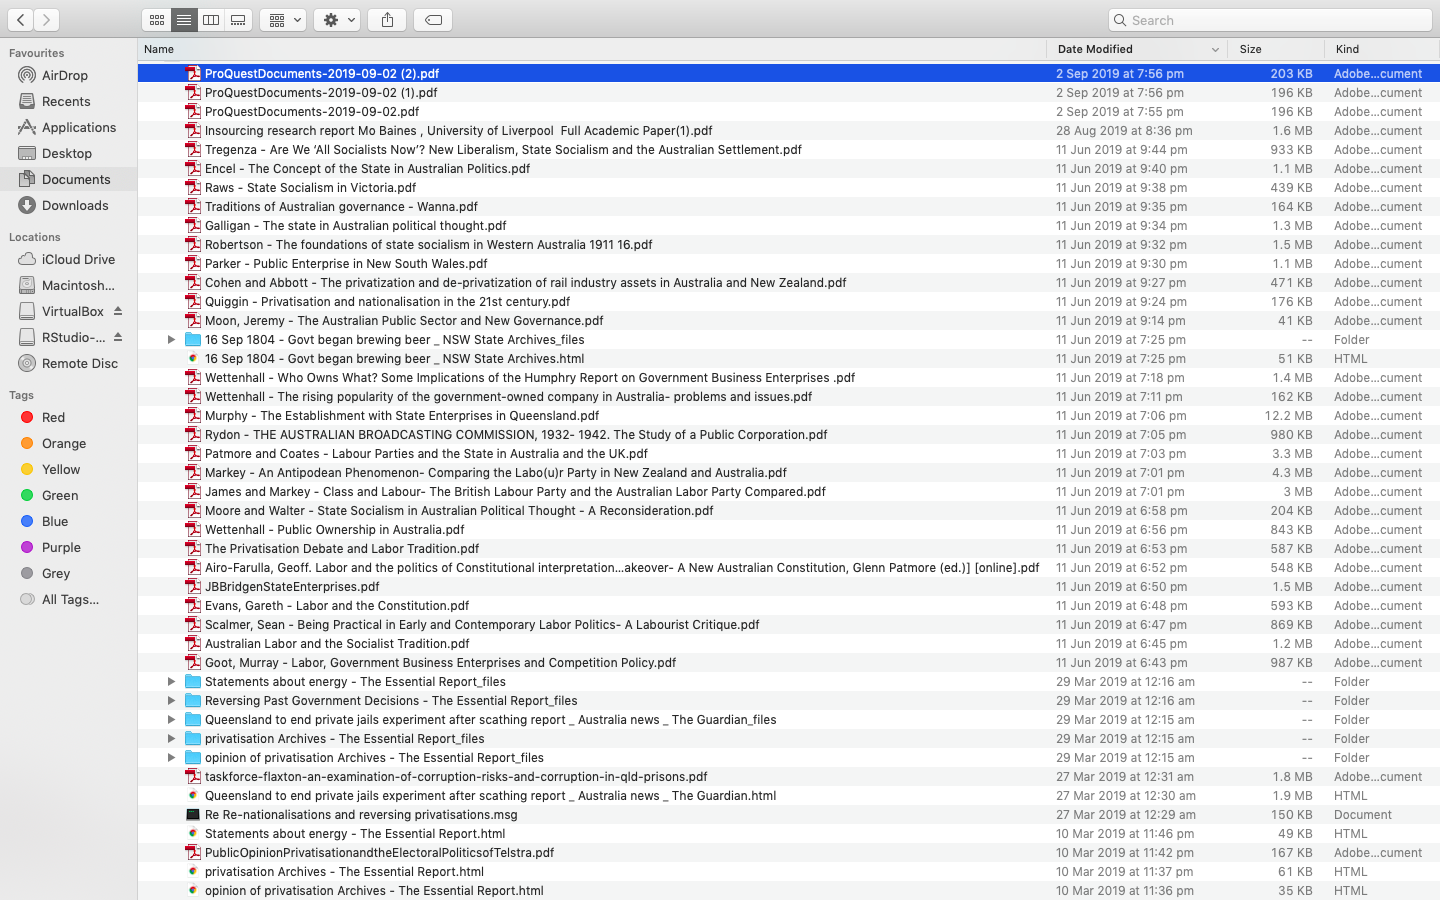
\includegraphics[width=1\textwidth,height=0.5\textheight,keepaspectratio]{pdf.png}\\

 \vspace{12pt}


 
   \end{column}
  \end{columns}

}

   
\end{frame}

\begin{frame}\label{\secvariable}
  %https://tex.stackexchange.com/a/7452/5483
    \parbox{\linewidth}{

\begin{columns}[t]
\begin{column}[c]{0.5\textwidth}
      
      I have written an installer for MacOS so you can access three tools using \href{https://github.com/MQ-FOAR705/Osmond-Chiu---Proof-of-Concept---Implementation.git}{\textbf{one download}}
 
      \vspace{12pt}
      
      Tool functions include annotation, tagging, search engine, reference management
      
      \vspace{12pt}
 
      It will save you time on tasks that could be better spent on improving your research!

 \end{column}
    \begin{column}[c]{0.5\textwidth}

 
 \includegraphics[width=1\textwidth,height=0.25\textheight,keepaspectratio]{figure/OpenSemanticSearch.png}\\
 \vspace{12pt}
 
\includegraphics[width=1\textwidth,height=0.25\textheight,keepaspectratio]{figure/Zotero.png}\\
\vspace{12pt}
 
\includegraphics[width=1\textwidth,height=0.25\textheight,keepaspectratio]{figure/Hypothesis.png}\\

   \end{column}
  \end{columns}
}
 
\end{frame}

%%%%%%%%%%%%%%%%%%%%%%%%%%%%%%%%%%%%%%%%%%%%%%%%%%%%%%%%%%%%%%%%%%%%%%%%%%
\mysection{radar}
%%%%%%%%%%%%%%%%%%%%%%%%%%%%%%%%%%%%%%%%%%%%%%%%%%%%%%%%%%%%%%%%%%%%%%%%%%
\begin{frame}\label{\secvariable}

What comprises the RBTools software package?

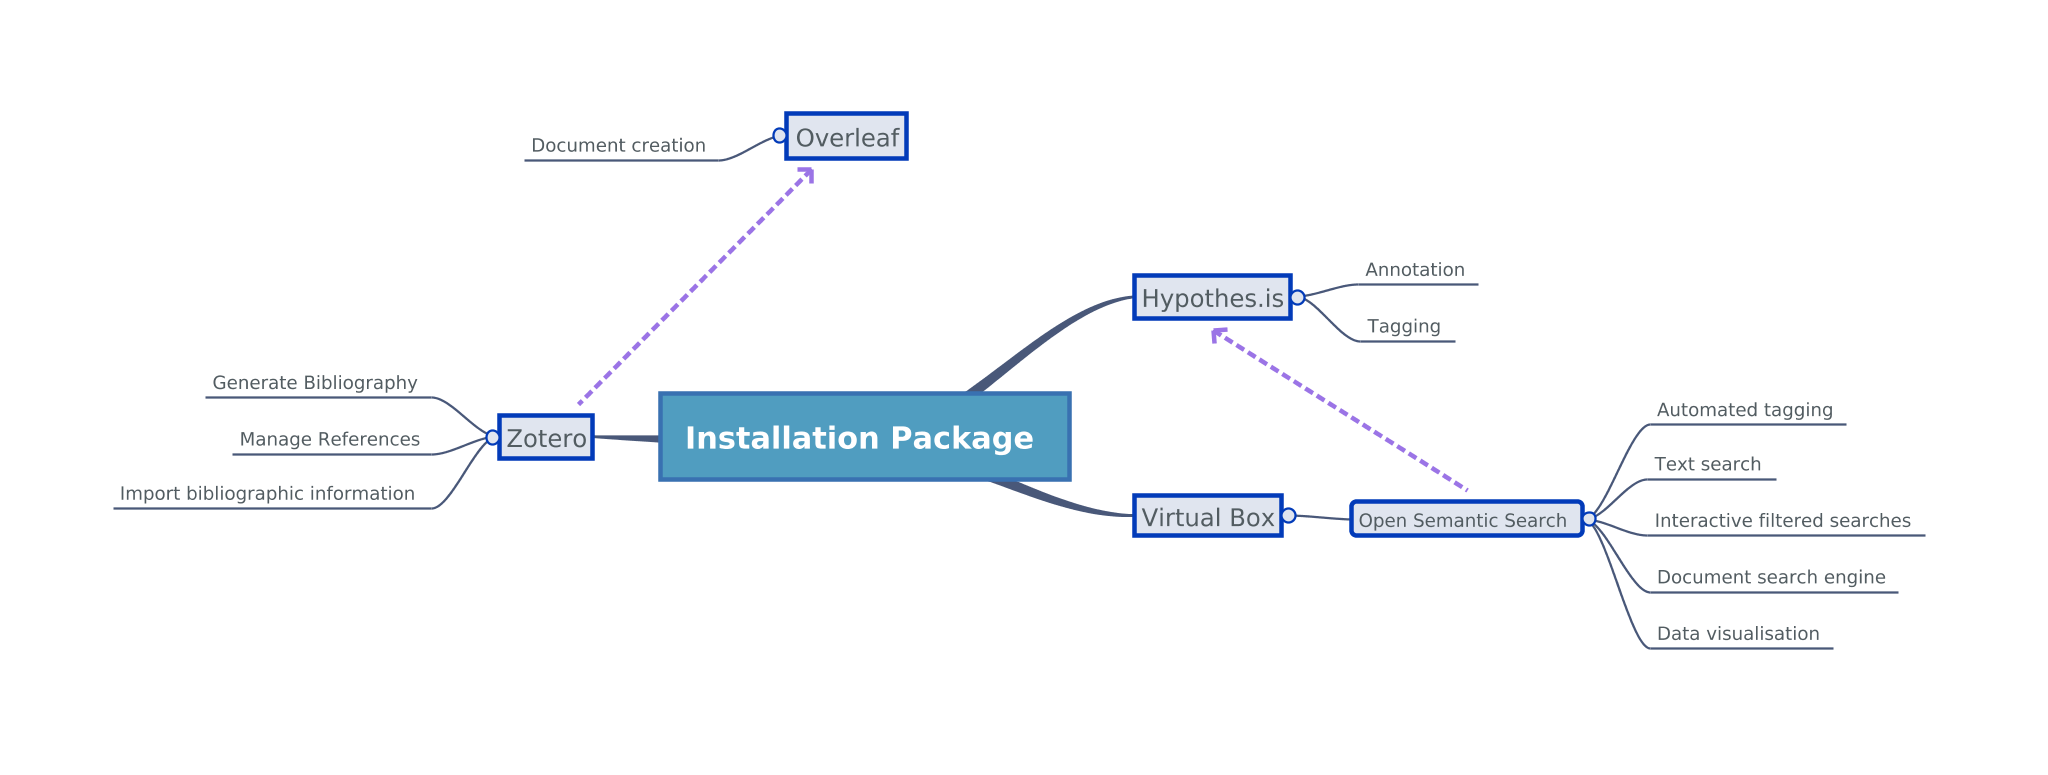
\includegraphics[width=1\textwidth,height=0.5\textheight,keepaspectratio]{%
figure/Pico.png}\\

Three useful, integrated tools for any researcher:
\begin{itemize}
    \item Zotero,
    \item Hypothes.is 
    \item Open Semantic Search.
    \end{itemize}

\end{frame}

%%%%%%%%%%%%%%%%%%%%%%%%%%%%%%%%%%%%%%%%%%%%%%%%%%%%%%%%%%%%%%%%%%%%%%%%%%
\mysection{line}
%%%%%%%%%%%%%%%%%%%%%%%%%%%%%%%%%%%%%%%%%%%%%%%%%%%%%%%%%%%%%%%%%%%%%%%%%%
\begin{frame}\label{\secvariable}

VirtualBox enables you to create a Virtual Machine where you can run another Operating System.
  \vspace{0.5cm}
  
  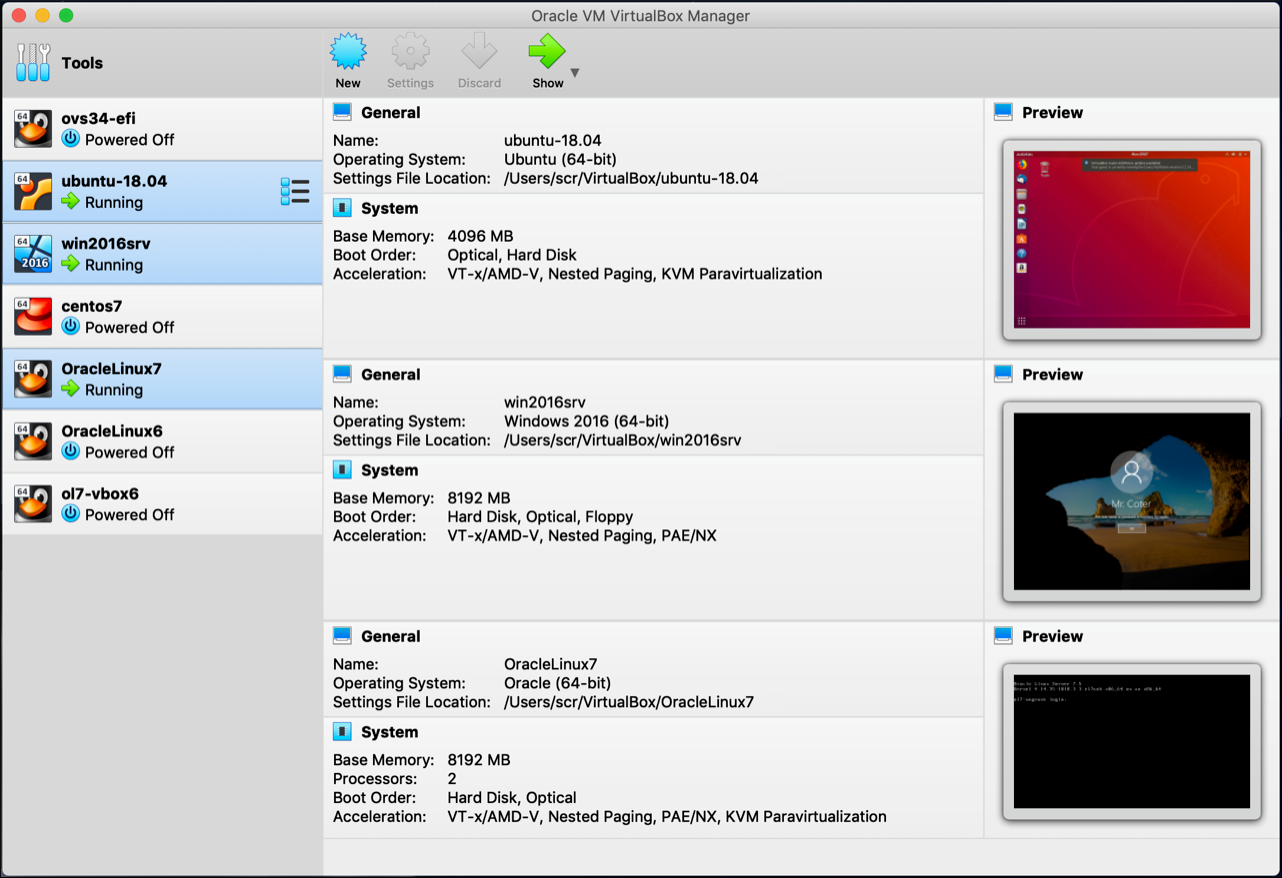
\includegraphics[width=1\textwidth,height=0.5\textheight,keepaspectratio]{%
figure/VirtualBox.png}\\  
\tiny Image by Oracle Corporation from \href{https://www.virtualbox.org/manual/}{Oracle® VM VirtualBox® User Manual}.

\end{frame}

%%%%%%%%%%%%%%%%%%%%%%%%%%%%%%%%%%%%%%%%%%%%%%%%%%%%%%%%%%%%%%%%%%%%%%%%%%
\mysection{major}
%%%%%%%%%%%%%%%%%%%%%%%%%%%%%%%%%%%%%%%%%%%%%%%%%%%%%%%%%%%%%%%%%%%%%%%%%%
\begin{frame}\label{\secvariable} %%Eine Folie
%http://lorempixel.com/1200/800/cats/Figure5/

Open Semantic Search is an integrated research tools for easier searching, monitoring, analytics, discovery and text mining of large document sets.
  \vspace{0.5cm}

\includegraphics[width=1\textwidth,height=0.5\textheight,keepaspectratio]{%
figure/OpenSemanticSearch.png}  

\tiny Image from \href{https://www.opensemanticsearch.org/doc/search}{Open Semantic Search}

\end{frame}

%%%%%%%%%%%%%%%%%%%%%%%%%%%%%%%%%%%%%%%%%%%%%%%%%%%%%%%%%%%%%%%%%%%%%%%%%%
\mysection{slab}
%%%%%%%%%%%%%%%%%%%%%%%%%%%%%%%%%%%%%%%%%%%%%%%%%%%%%%%%%%%%%%%%%%%%%%%%%%
\begin{frame}\label{\secvariable}

Zotero is an open-source reference and bibliography management tool.
  \vspace{0.5cm}

\includegraphics[width=1\textwidth,height=0.5\textheight,keepaspectratio]{%
figure/Zotero.png}

\tiny Image from \href{https://www.zotero.org/}{Zotero}


\end{frame}





%%%%%%%%%%%%%%%%%%%%%%%%%%%%%%%%%%%%%%%%%%%%%%%%%%%%%%%%%%%%%%%%%%%%%%%%%%
\mysection{minor}
%%%%%%%%%%%%%%%%%%%%%%%%%%%%%%%%%%%%%%%%%%%%%%%%%%%%%%%%%%%%%%%%%%%%%%%%%%
\begin{frame}\label{\secvariable} %%Eine Folie

Hypothes.is is an annotation tool for digital documents.
  \vspace{0.5cm}

\includegraphics[width=1\textwidth,height=0.7\textheight,keepaspectratio]{%
figure/Hypothesis.png}

\tiny Image from \href{https://web.hypothes.is/annotation-tips-for-students/}{Annotation Tips} for Students by Hypothes.is 

\end{frame}

%%%%%%%%%%%%%%%%%%%%%%%%%%%%%%%%%%%%%%%%%%%%%%%%%%%%%%%%%%%%%%%%%%%%%%%%%%
\mysection{conclusion}
%%%%%%%%%%%%%%%%%%%%%%%%%%%%%%%%%%%%%%%%%%%%%%%%%%%%%%%%%%%%%%%%%%%%%%%%%%
\begin{frame}\label{\secvariable}
  
With RBTools, you will be able to  
  \begin{itemize}
   \item annotate, highlight and tag webpages. 
  \item apply a search engine to index documents, automatically tag documents, search and text mine its contents, do analytics and data visualisations.
  \item create and manage references and bibliographies for any text editor and directly inside programs.

  \end{itemize}

  \vspace{0.5cm}

You can download the RBTools installer and instructions from \href{https://github.com/MQ-FOAR705/Osmond-Chiu---Proof-of-Concept---Implementation}{https://github.com/MQ-FOAR705/Osmond-Chiu---Proof-of-Concept---Implementation}

\end{frame}



\end{document}
